\documentclass[english, a4paper,12pt]{article}
\usepackage[a4paper, top=2cm, bottom=2cm,right=2cm,left=2cm]{geometry}
\date{} 
\usepackage{tikz}
\usepackage[utf8]{vietnam}
\usepackage{textcomp, graphicx, titling, tkz-tab, changepage}
\usepackage{changepage, amsmath, fancyvrb, minted, caption} 
\usepackage{booktabs}
\usepackage{tabularx}
\usepackage{amsfonts} 
\usepackage[dvipsnames]{xcolor}
\usepackage[english]{babel}
\usepackage{listings}
\usepackage{svg}
\usepackage{hyperref}
\hypersetup{
    colorlinks=true,
    linkcolor=black,
    filecolor=magenta,      
    urlcolor=Green,
    pdftitle={Overleaf Example},
    pdfpagemode=FullScreen,
    }
\definecolor{LightGray}{gray}{0.95}


\addto\captionsenglish{
  \renewcommand{\contentsname}
  {Table of Contents}
}

\begin{document}
\begin{titlepage}
\begin{center}
\textbf{UNIVERSITY OF INFORMATION TECHNOLOGY}

\textbf{FACULTY OF COMPUTER SCIENCE}

\vspace{1cm}

\vspace{1cm}

\textbf{Deep Deterministic Policy Gradient (DDPG) \& Twin-Delayed DDPG (TD3)}

\vspace{2cm}
\includegraphics[width= 5cm]{logo.png}
\vspace{2cm}

\textbf{Instructor: } Luong Ngoc Hoang

\vspace{0.5cm}

\textbf{Student:} Ha Huy Hoang - 22520460
\vspace{0.5cm}
\\
\textbf{Class:} CS211.P11
\vspace{2cm}
\tableofcontents
\end{center}
\end{titlepage}

\section*{1. Introduction}
\addcontentsline{toc}{section}{1. Introduction}
\hspace*{5mm} $\textbf{DDPG}^{[1]} $(Deep Deterministic Policy Gradient) is an actor-critic algorithm that extends DQN to handle continuous action spaces. It uses deterministic policy gradient theorem to train a deterministic policy. DDPG employs two networks: an actor network that outputs actions and a critic network that estimates Q-values. Like DQN, it uses experience replay and target networks to stabilize training, but adds noise to actions during exploration.
\\
\vspace*{-5mm}
\\
\hspace*{5mm} The actor and critic updates in DDPG pseudocode follow:
\begin{center}
    \includesvg[width=0.6\linewidth]{pseudocode_of_ddpg.svg}
\end{center}
\vspace*{-2mm}

\hspace*{5mm}$\textbf{TD3}^{[2]}$ (Twin Delayed Deep Deterministic Policy Gradient) is an enhancement to DDPG that addresses overestimation bias and improves training stability. It introduces three major modifications: clipped Double-Q Learning, delayed policy updates and target policy smoothing. The clipped Double-Q Learning using the smaller Q-value for the target, and regressing towards that, helps fend off overestimation in the Q-function; while delayed policy updates and noise addition to target actions further stabilize training.\\
\hspace*{5mm} TD3 concurrently learns two Q-functions, $Q_{\phi_1}$ and $Q_{\phi_2}$, by mean square Bellman error minimization, in almost the same way that DDPG learns its single Q-function. 
\begin{itemize}
    \vspace*{-2mm}
    \item \textbf{Target Policy Smoothing:} 
    \vspace*{-2mm}
    \begin{itemize}
        \item Adds clipped noise to target actions: $\mu'(s') + \epsilon$, where $\epsilon \sim \text{clip}(\mathcal{N}(0, \sigma), -c, c)$.
        \item Acts as a regularizer to prevent the policy from exploiting incorrect peaks in the Q-function.
        \item Smooths out the Q-function over similar actions for more stable learning.
    \end{itemize}
    \vspace*{-4mm}
    \item \textbf{Clipped Double-Q Learning:}
    \vspace*{-2mm}
    \begin{itemize}
        \item Uses two Q-functions instead of one.

        \item Takes the minimum Q-value between the two critics for target calculation:
            \begin{center}
                \includesvg[width=0.4\linewidth]{clip_double.svg}
            \end{center}
                \begin{flushright}
        \vspace*{-1mm}
        \scriptsize [1]: \href{https://spinningup.openai.com/en/latest/algorithms/ddpg.html}{Deep Deterministic Policy Gradient}\\
        \scriptsize [2]: \href{https://spinningup.openai.com/en/latest/algorithms/td3.html}{Twin Delayed DDPG}
        \end{flushright}
        \item Both Q-functions are trained using this same target.
        \item Helps prevent overestimation bias common in DDPG.
    \end{itemize}
    \vspace*{-2mm}
    \item \textbf{Delayed Policy Updates:}
    \vspace*{-2mm}
    \begin{itemize}
        \item Policy network is updated less frequently than Q-functions.
        \item Typically updated once for every 2-3 Q-function updates.
        \item Reduces volatility in training by allowing Q-functions to converge more before policy updates.
    \end{itemize}
\end{itemize}
\begin{center}
    \includesvg[width=0.6\linewidth]{pseudocode_of_td3.svg}
\end{center}
\vspace*{-7mm}
\section*{2. Statistics}
\addcontentsline{toc}{section}{2. Statistics}
\hspace*{5mm} As the teacher has guided, I will use TensorBoard to compare different runs. However, there is an issue with large fluctuations between steps, making the graphs difficult to read and analyze. Therefore, I have adjusted the smoothing to 0.99 to make the analysis easier. Since the second neural network of TD3 is only used for cross-checking with the first neural network, helping to evaluate the value of actions more accurately, it has no value in analysis as it is not compared with DDPG (using the first neural network for comparison, therefore in the report will not comment on these graphs).
\\
\hspace*{5mm}  Each color lines presents a algorithm with seed that have the structer likes algorithm\_seed, the seeds and algorithm i used for experiment is listed below:

\begin{center}
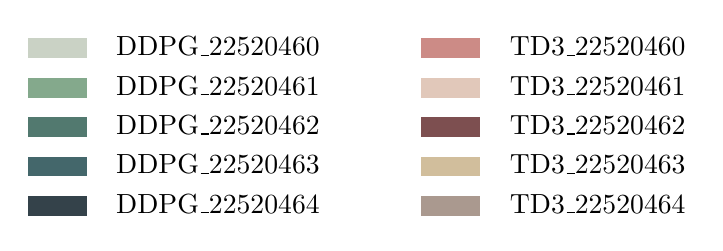
\begin{tikzpicture}
    % Định nghĩa các màu mới
    \definecolor{color10}{RGB}{170,153,143} % Màu #aa998f
    \definecolor{color9}{RGB}{209,190,156} % Màu #d1be9c
    \definecolor{color8}{RGB}{125,79,80}   % Màu #7d4f50
    \definecolor{color7}{RGB}{225,200,186} % Màu #e1c8ba
    \definecolor{color6}{RGB}{204,139,134} % Màu #cc8b86
    \definecolor{color5}{RGB}{52,66,74}    % Màu #34424a
    \definecolor{color4}{RGB}{68,103,107}  % Màu #44676b
    \definecolor{color3}{RGB}{82,121,111}  % Màu #52796f
    \definecolor{color2}{RGB}{132,169,140} % Màu #84a98c
    \definecolor{color1}{RGB}{202,210,197} % Màu #cad2c5

    % ------------------------
    % Cột trái: 5 màu đầu
    % ------------------------
    % Hình chữ nhật màu #cad2c5 (ddpg_22520460)
    \fill[color1] (0,0) rectangle (0.75,0.25); % Tô màu #cad2c5
    \node[right] at (1,0.15) {DDPG\_22520460};

    % Hình chữ nhật màu #84a98c (ddpg_22520461)
    \fill[color2] (0,-0.5) rectangle (0.75,-0.25); % Tô màu #84a98c
    \node[right] at (1,-0.35) {DDPG\_22520461};

    % Hình chữ nhật màu #52796f (ddpg_22520462)
    \fill[color3] (0,-1) rectangle (0.75,-0.75); % Tô màu #52796f
    \node[right] at (1,-0.85) {DDPG\_22520462};

    % Hình chữ nhật màu #44676b (ddpg_22520463)
    \fill[color4] (0,-1.5) rectangle (0.75,-1.25); % Tô màu #44676b
    \node[right] at (1,-1.35) {DDPG\_22520463};

    % Hình chữ nhật màu #34424a (ddpg_22520464)
    \fill[color5] (0,-2) rectangle (0.75,-1.75); % Tô màu #34424a
    \node[right] at (1,-1.85) {DDPG\_22520464};

    % ------------------------
    % Cột phải: 5 màu sau
    % ------------------------
    % Hình chữ nhật màu #cc8b86 (td3_22520460)
    \fill[color6] (5,0) rectangle (5.75,0.25); % Tô màu #cc8b86
    \node[right] at (6,0.15) {TD3\_22520460};

    % Hình chữ nhật màu #e1c8ba (td3_22520461)
    \fill[color7] (5,-0.5) rectangle (5.75,-0.25); % Tô màu #e1c8ba
    \node[right] at (6,-0.35) {TD3\_22520461};

    % Hình chữ nhật màu #7d4f50 (td3_22520462)
    \fill[color8] (5,-1) rectangle (5.75,-0.75); % Tô màu #7d4f50
    \node[right] at (6,-0.85) {TD3\_22520462};

    % Hình chữ nhật màu #d1be9c (td3_22520463)
    \fill[color9] (5,-1.5) rectangle (5.75,-1.25); % Tô màu #d1be9c
    \node[right] at (6,-1.35) {TD3\_22520463};

    % Hình chữ nhật màu #aa998f (td3_22520464)
    \fill[color10] (5,-2) rectangle (5.75,-1.75); % Tô màu #aa998f
    \node[right] at (6,-1.85) {TD3\_22520464};

\end{tikzpicture}
\end{center}


\newpage
\subsection*{2.1. HalfCheetah-v4}\addcontentsline{toc}{subsection}{2.1. HalfCheetah-v4}

\includegraphics[width=6cm]{SPS_hf.png}
\includegraphics[width=6cm]{episodic_length_hf.png}
\includegraphics[width=6cm]{episodic_return_hf.png}
\includegraphics[width=6cm]{actor_loss_hf.png}
\includegraphics[width=6cm]{qf1_loss_hf.png}
\includegraphics[width=6cm]{qf1_values_hf.png}
\includegraphics[width=6cm]{qf2_loss_hf.png}
\includegraphics[width=6cm]{qf2_values_hf.png}
\includegraphics[width=6cm]{qf_loss_hf.png}
\begin{center}
    \textbf{Figure 1.} HalfCheetah-v4
\end{center}
\hspace*{5mm} Looking at the first chart, we can see that the SPS of TD3 is consistently lower than that of DDPG. The SPS of TD3 ranges from approximately 180 to 200, while DDPG's ranges from 240 to 250 (both trained on the same NVIDIA TESLA P100 GPUs configuration on Kaggle). TD3 has a lower SPS compared to DDPG because it uses a more complex architecture with two Critics networks (instead of one like DDPG), along with mechanisms such as delayed updates and target policy smoothing, resulting in more computations required for each training step.
\\
\vspace*{-2mm}
\\
\hspace*{5mm}The episodic length just witnessed one value 1000 because the episode truncates when the length of the episode is greater than 1000$^{[3]}$. In terms of episodic return, both show an upward trend in scores (return) over the course of training.
\\
\vspace*{-2mm}
\\
\hspace*{5mm}TD3 has a higher actor loss because it updates the actor less frequently (delayed policy update) and uses min($Q_1$, $Q_2$) for policy updates, resulting in more cautious learning. In this case, based on the rewards graph (qf1\_values), it shows that DDPG (blue) achieves higher values compared to TD3 (red). The mechanisms in TD3 to prevent overestimation (using min Q-values and target policy smoothing) may be overly cautious and unnecessary in this specific training environment, leading to lower performance than DDPG (in some seed TD3 shows the much higher qf1\_loss than DDPG). This indicates that although TD3 is designed to address the shortcomings of DDPG, these improvements do not always result in better performance in every environment.
\begin{flushright}
\scriptsize [3]: \href{https://www.gymlibrary.dev/environments/mujoco/half_cheetah/}{Half Cheetah - Gym Documentation}
\end{flushright}
\newpage
\subsection*{2.2. Ant-v4}\addcontentsline{toc}{subsection}{2.2. Ant-v4}

\includegraphics[width=6cm]{SPS_ant.png}
\includegraphics[width=6cm]{episodic_length_ant.png}
\includegraphics[width=6cm]{episodic_return_ant.png}
\includegraphics[width=6cm]{actor_loss_ant.png}
\includegraphics[width=6cm]{qf1_loss_ant.png}
\includegraphics[width=6cm]{qf1_values_ant.png}
\includegraphics[width=6cm]{qf2_loss_ant.png}
\includegraphics[width=6cm]{qf2_values_ant.png}
\includegraphics[width=6cm]{qf_loss_ant.png}
\begin{center}
    \textbf{Figure 2.} Ant-v4
\end{center}

\hspace*{5mm}As mentioned in the earlier context, TD3 consistently has a lower SPS compared to DDPG. This is due to its more intricate architecture featuring two Critics networks (unlike DDPG, which uses only one), along with techniques such as delayed updates and target policy smoothing, leading to increased computational demands for each training step.
\\
\vspace*{-2mm}
\\
\hspace*{5mm} However, in the Ant-v4 environment, we observe a difference in the episodic length and episodic return produced by the two algorithms. In both charts representing these values, TD3 consistently shows higher values, indicating superior performance in this environment. Specifically, the episodic length of TD3 converges much faster than DDPG, reaching 1000$^{[4]}$ (the termination condition of the environment if the Ant is considered "healthy") without smoothing, while DDPG fluctuates between 400 and 750. Additionally, the rewards returned by TD3 are significantly higher than those of DDPG (ranging from 4000 to 5800 compared to 600 to 2500). From this, we can conclude that TD3 outperforms DDPG in the Ant-v4 environment.
\\
\vspace*{-2mm}
\\
\hspace*{5mm} In terms of actor\_loss, both show a downward trend in loss over the course of training. In contrast, the qf1\_loss of TD3 becomes lower than that of DDPG toward the end of training. In the qf1\_values chart, we observe that TD3 has higher values compared to DDPG in most seeds. This may be because, in a complex environment like Ant-v4, DDPG is more prone to getting stuck in local optima due to overestimation, whereas TD3’s more cautious mechanisms (min Q-values, delayed policy update) help it discover better policies.
\begin{flushright}
\scriptsize [4]: \href{https://www.gymlibrary.dev/environments/mujoco/ant/}{Ant - Gym Documentation}
\end{flushright}
\newpage

\section*{3. Conclusion}
\addcontentsline{toc}{section}{3. Conclusion}
\hspace*{5mm} All the algorithms and seed i runned with this tempalte command:
\begin{minted}[bgcolor=LightGray, fontsize=\footnotesize]{Python}
python cleanrl/algo.py --seed seed --env-id game --total-timesteps 2000000 --capture_video
\end{minted}
\hspace*{5mm} There is an issue with capturing videos where only the first video is recorded properly, and the remaining videos appear black. I searched for solutions online but couldn’t find any, so I added an episodic trigger to capture a video at episode 1999. Why episode 1999? Because the total-timesteps I used is 2,000,000, and the maximum timesteps for each episode in both environments is 100,000. Thus, I chose to record the video at the final episode in the hope that it would capture the best performance. The best videos of each algorithm in environments are stored in this \href{https://drive.google.com/drive/folders/1QlgdHN7lEf0Oh_XfwRc2fczze2t9ugJU?usp=sharing}{link}.
\\
\vspace*{-2mm}
\\
\hspace*{5mm} In less complex environments like HalfCheetah-v4, the performance charts of DDPG and TD3 are almost equivalent. However, based on my subjective evaluation, the result videos of DDPG across all seeds are not as good. This is because agents in DDPG tend to run too fast and sometimes stumble, whereas TD3 does not exhibit this issue.
\\
\vspace*{-2mm}
\\
\hspace*{5mm} In more complex environments like Ant-v4, DDPG's performance charts and result videos are significantly worse compared to TD3. In some videos, the agents using DDPG run normally for a short distance and then flip over, remaining that way for the rest of the timesteps (as the center height z does not reach the threshold, so it isn't truncated)(I will choose the best video based solely on the agent's running time without considering the timesteps). In other cases, the agents become "unhealthy" during the run and are stopped (and from a personal perspective, the agent moves quite slowly and a relatively short distance compared to TD3). On the other hand, in TD3's videos, the agents consistently run normally without such problems.
\\
\vspace*{-2mm}
\\
\hspace*{5mm} In summary, we can trade off the relatively small differences in the performance of the two algorithms in less complex environments like HalfCheetah-v4 for faster training by using DDPG. However, in more complex environments like Ant-v4, choosing TD3 is more reasonable because the training time is not significantly different, but the performance is substantially better compared to DDPG. A comprehensive list of results performed by the authors of the TD3 paper is available on page 7 of the \href{https://arxiv.org/pdf/1802.09477}{paper}

\end{document}
